\documentclass[11pt]{article}
\usepackage[english]{babel}
\usepackage{graphicx}
\graphicspath{{images/}}
\usepackage{vmargin}
\usepackage{enumitem}               % ridefinisce la spaziatura nelle liste
\setlist{topsep=5px, itemsep=3px}
\usepackage{hyperref}
\usepackage{multicol}
\usepackage{float}
\usepackage{subcaption}
\usepackage{caption}

\hypersetup{
    colorlinks=true,
    linkcolor=black,        % color of internal links
    citecolor=black,        % color of links to bibliography
    filecolor=blue,         % color of file links
    urlcolor=blue,          % color of external links
}
\setmarginsrb{3 cm}{1 cm}{3 cm}{2.5 cm}{1 cm}{1.5 cm}{1 cm}{1.5 cm}
\usepackage{multirow}
\usepackage{enumitem}

\date{A.Y. 2020-2021}

\makeatletter
\def\projectName{Binary Functions Classification}
\let\documentTitle\@title    
\let\academicYear\@date
\makeatother

\begin{document}
\begin{titlepage}
	\centering
    \vspace*{0.5 cm}
    \textsc{\LARGE Foundations of Data Science}\\[0.2 cm]
    \textsc{\Large Final Project}\\[0.5 cm]
	\textsc{\textit{La Sapienza University}, Computer Science}\\[0.25 cm]
	\textsc{\academicYear}\\[0.75 cm]
	\rule{\linewidth}{0.2 mm} \\[0.4 cm]
	\textsc{\Huge \projectName}\\
	%\rule{\linewidth}{0.2 mm} \\[0.4 cm]
	%\textsc{\large \documentTitle}\\
	\rule{\linewidth}{0.2 mm} \\[0.4 cm]
	
	\large
	Andrea Gasparini, \texttt{1813486}\\[0.2 cm]
    Edoardo Di Paolo, \texttt{1728334}\\[0.2 cm]
    Cirillo Atalla, \texttt{1755033}\\[0.2 cm]
    
    \tableofcontents
\end{titlepage}

\newpage

\section{Introduction}
The task of this project was to build a \textit{multiclass} classifier to determine whether an assembly function is an \textbf{encryption}, \textbf{math}, \textbf{string manipulation} or \textbf{sorting} function. Formally, the task was to approximate a mapping function:
\[ f : X_{bin} \rightarrow \{encryption, math, string, sort\} \]
where $X_{bin}$ is an assembly set of instructions that can be classified in one of the target classes of the $f$ function's right-hand side. To be more precise, since we have to define a features list to train a Machine Learning model, $X_{bin}$ is a list of measurable properties extracted from the dataset after a feature extraction procedure.

\section{Motivations}
The functions classification is a useful task, for example, in the \textit{malware analysis}. Certain Machine Learning models are able to understand when a program is a malware or not doing a binary classification. These Machine Learning models are useful also in the process of \textit{reverse engineering} because in an unknown software it is often useful to find specific functions.

\section{Evaluation methods}
In order to evaluate a solution based on a features list, it's necessary to train some models and compare the performances according to some metrics. The comparisons in this report are based on the results obtained from three models: \textbf{Decision Tree}, \textbf{Support Vector Machine} and \textbf{Logistic Regression}. We used different metrics to evaluate the performances of these models, like plotting the \textit{confusion matrices} and comparing \textit{precision}, \textit{recall} and \textit{f1-score}. Another metric that we took in consideration was the way of splitting the dataset; in fact the standard way is to reserve $\frac{2}{3}$ for the training and $\frac{1}{3}$ for the test. Decreasing the first one and therefore increasing the second one could get worse performances, but if we still get acceptable results it probably means that the chosen features are meaningful.

\section{Dataset, preprocessing and features extraction}
The initial dataset had \textbf{14397} assembly functions containing \textit{duplicates}. Then we removed all the duplicates and we got \textbf{6073} functions. As we can see in \autoref{fig:nodupdataset}, removing the duplicates creates an unbalanced dataset and this can lead to problems such as predicting the minority class.

\begin{figure}[H]
\centering
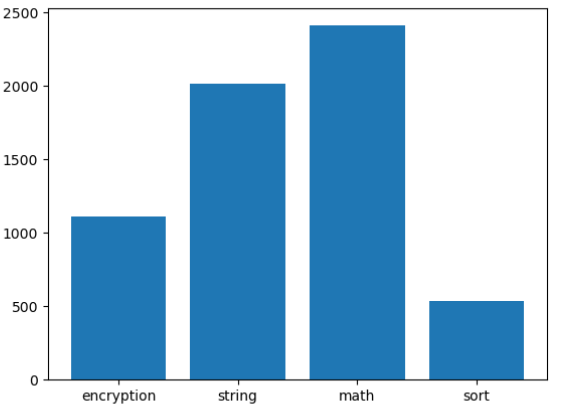
\includegraphics[scale=0.4]{images/dataset_without_dup.png}
\caption{Dataset without duplicates}
\label{fig:nodupdataset}
\end{figure}

Each entry of the dataset, provided as a JSON, represent an assembly function and contains:
\begin{itemize}
    \item the label of the function, that is one of the target classes;
    \item the linear list of his assembly instructions;
    \item the control flow graph (CFG), encoded as a NetworkX graph.
\end{itemize}

Every entry in the dataset has been processed and mapped in a list with these following features:
\begin{multicols}{2}
    \begin{itemize}
        \item \textit{graph\_nodes}: it is the number of nodes in the CFG;
        \item \textit{graph\_diam}: it is the maximum diameter value of the CFG's strongly connected components;
        \item \textit{mov}: it is the number of mov instructions in the function;
        \item \textit{bitwise}: it is the number of bitwise instructions in the function;
        \item \textit{xmm}: it is the number of xmm registers in the function;
        \item \textit{arithm}: it is the number of arithmetic instructions in the function;
        \item \textit{cmp}: it is the number of cmp instructions in the function;
        \item \textit{shift}: it is the number of shift instructions in the function;
        \item \textit{calls}: it is the number of calls instructions in the function;
        \item \textit{cyclomatic complexity}: the cyclomatic complexity of the CFG.
    \end{itemize} 
\end{multicols}

\section{Results and conclusions}
The \textit{Decision Tree} model obtains the best results compared to \textit{SVM} and \textit{Logistic Regression}. The bigger issue was the misclassification of \textit{sort} functions because in the dataset we have a small number of these functions. Incrementing the number of \textit{sort} instances in dataset without adding duplicates would certainly improve the performances for these cases, but produce this new data could require a lot of effort.
\newpage

\begin{figure}
\centering
\begin{subfigure}{.5\textwidth}
  \centering
  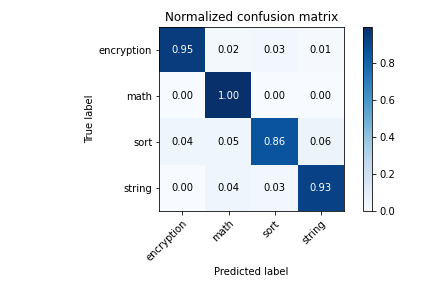
\includegraphics[width=1\linewidth]{svm_30_70.png}
  \caption{SVM with 33\% test}
  \label{fig:svm}
\end{subfigure}%
\begin{subfigure}{.5\textwidth}
  \centering
  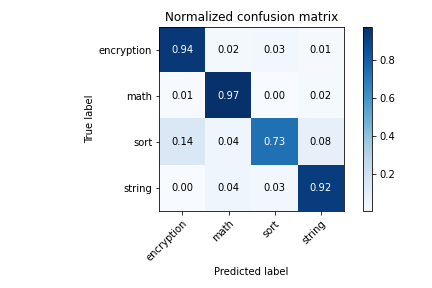
\includegraphics[width=1\linewidth]{regression_30_70.png}
  \caption{Logistic Regression with 33\% test}
  \label{fig:logreg}
\end{subfigure}
\begin{subfigure}{.5\textwidth}
  \centering
  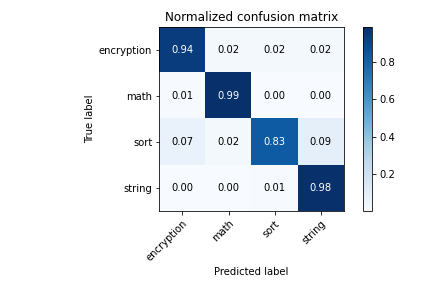
\includegraphics[width=1\linewidth]{decision_tree_30_70.png}
  \caption{Decision Tree with 33\% test}
  \label{fig:dectree}
\end{subfigure}%
\label{fig:test}
\end{figure}

In these images there are the results that we obtain with each method with a test size equal to the 33\% of the dataset. Here we have the tables with the different metrics we obtained for each method.

\begin{table}[h]
\centering
\begin{tabular}{|l|l|l|l|l|}
\hline
             & precision & recall & f1-score & support \\ \hline
encryption   & 0.98      & 0.95   & 0.96     & 366     \\ \hline
math         & 0.95      & 1.00   & 0.97    & 816     \\ \hline
sort         & 0.83     & 0.86   & 0.84     & 173     \\ \hline
string       & 0.98      & 0.93   & 0.95     & 650     \\ \hline
             &           &        &          &         \\ \hline
accuracy     &           &        & 0.95     & 2005    \\ \hline
macro avg    & 0.93      & 0.93   & 0.93     & 2005    \\ \hline
weighted avg & 0.95      & 0.95   & 0.95    & 2005    \\ \hline
\end{tabular}
\caption{Decision Tree metrics.}
\end{table}

\begin{table}[h]
\centering
\begin{tabular}{|l|l|l|l|l|}
\hline
             & precision & recall & f1-score & support \\ \hline
encryption   & 0.94      & 0.94   & 0.94     & 366     \\ \hline
math         & 0.98      & 0.99   & 0.99     & 816     \\ \hline
sort         & 0.92      & 0.83   & 0.87     & 173     \\ \hline
string       & 0.96      & 0.98   & 0.97     & 650     \\ \hline
             &           &        &          &         \\ \hline
accuracy     &           &        & 0.97     & 2005    \\ \hline
macro avg    & 0.95      & 0.94   & 0.94     & 2005    \\ \hline
weighted avg & 0.96      & 0.97   & 0.96     & 2005    \\ \hline
\end{tabular}
\caption{SVM metrics.}
\end{table}

\begin{table}[h]
\centering
\begin{tabular}{|l|l|l|l|l|}
\hline
             & precision & recall & f1-score & support \\ \hline
encryption   & 0.91      & 0.94   & 0.92     & 366     \\ \hline
math         & 0.95      & 0.99   & 0.99     & 816     \\ \hline
sort         & 0.81      & 0.73   & 0.77     & 173     \\ \hline
string       & 0.95      & 0.92   & 0.94     & 650     \\ \hline
             &           &        &          &         \\ \hline
accuracy     &           &        & 0.93     & 2005    \\ \hline
macro avg    & 0.90      & 0.89   & 0.90     & 2005    \\ \hline
weighted avg & 0.93      & 0.93   & 0.93     & 2005    \\ \hline
\end{tabular}
\caption{Logistic regression metrics.}
\end{table}

\end{document}